\chapter{Aplicación}
\section{Introducción}
La Capa de Aplicación muestra los servicios de aplicación que apoyan el negocio, y las aplicaciones que los realizan.
El principal elemento de estructura activa de la Capa de Aplicación es el componente de aplicación. Este elemento se utiliza para modelar cualquier entidad estructural en la Capa de Aplicación: no sólo los componentes de software (reutilizables) que pueden formar parte de una o más aplicaciones, sino también las aplicaciones de software completas, las subaplicaciones o los sistemas de información. Aunque es muy similar al UML componente, el elemento componente de la aplicación ArchiMate modela estrictamente el aspecto estructural de una aplicación; su comportamiento está modelado por una relación explícita con el elemento de comportamiento.
También en la arquitectura de aplicación, las interrelaciones de los componentes son un ingrediente esencial. Por lo tanto, también introducimos aquí el elemento de colaboración de la aplicación, definido como un colectivo de componentes de aplicación que realizan interacciones de aplicación. El elemento es muy similar a la colaboración como se define en el estándar UML.
En el sentido puramente estructural, una interfaz de aplicación es el canal (lógico) a través del cual se puede acceder a los servicios de un componente. En un sentido más amplio (tal como se utiliza, entre otros, en la definición de UML), una interfaz de aplicación define algunas características de comportamiento elementales: define el conjunto de operaciones y eventos que proporciona el componente, o los que se requieren del entorno. Así, se utiliza para describir la funcionalidad de un componente. El elemento de interfaz de aplicación puede utilizarse para modelar tanto las interfaces de aplicación a aplicación, que ofrecen servicios de aplicación internos, como las interfaces de aplicación a empresa (y/o interfaces de usuario), que ofrecen servicios de aplicación externos.

\section{Metamodelo}
\begin{figure}[h!]
	\centering
	\includegraphics[width=0.9\linewidth]{imgs/meta/Aplicacion}
	\caption{Metamodelo Aplicación}
\end{figure}

La figura 7.1 brinda una visión general de los elementos de la capa de aplicación y sus relaciones. Siempre que sea aplicable, la guía se ha extraído de la analogía con la Capa de Aplicación. La Capa de Aplicación se utiliza típicamente para modelar las arquitecturas de los sistemas de información de la empresa, incluida la arquitectura de aplicación que, como se define en el marco del TOGAF, describe la estructura e interacción de las aplicaciones. Un componente de aplicación representa una encapsulación de la funcionalidad de la aplicación alineada con la estructura de implementación, que es modular y reemplazable. Encapsula su comportamiento y datos, expone los servicios y los hace disponibles a través de interfaces.

\newpage
\chapter{Comportamiento}
\section{Introduccion}
contenido...

\newpage
\section{Punto de Vista de Cooperación de Actor}


\subsection{Modelo de Cooperación de Actor}
\begin{figure}[h!]
	\centering
	\includegraphics[width=.6\linewidth]{imgs/modelo/CoopActor.pdf}
	\caption{Modelo Cooperacion de Actor}
\end{figure}

El punto de vista de cooperación de actor establece las colaboraciones que existen internamente y externamente sobre un actor o rol de la organización con el fin de mostrar de qué manera interactuan e interfiere con el actor en cuestión. Por medio de interfaces  que comunican los entes del exterior y el interior de la organización con el actor o rol.

\newpage
\subsection{Caso  de Cooperación de Actor}
\begin{figure}[h!]
	\centering
	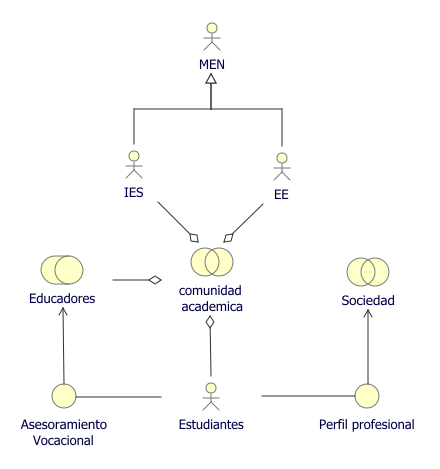
\includegraphics[width=.8\linewidth]{imgs/caso/negocio/coperacion_actor.pdf}
	\caption{Caso Cooperacion de Actor}
\end{figure}

Para nuestro objeto de estudio en relación al punto de vista de colaboración de actor tenemos como actor principal a los estudiantes aquellos que colaboran en la comunidad académica y hacen parte de las IES y EE que son regidas por el Ministerio de Educación. Por otro lado tenemos el rol de educador que hace parte de la comunidad y que puede ayudar a guiar en parte la vocación que construirá en un futuro el estudiante. Los estudiantes contribuirán en la sociedad gracias a su perfil que se ha formado durante sus años de estudio y que permitirán a las empresas apoderarse de estos individuos y así lograr mejores avances que colaboren en su entidad y por tanto a la sociedad misma.

\newpage
\section{Punto de Vista Estructura de Información}
Una estructura de información es una estructura jerárquica centrada en el producto que organiza la información relacionada con un producto o biblioteca. Dentro de una estructura de información, los subgrupos de información denominados grupos de información organizan el contenido. Estos objetos de contenido se denominan elementos de información. Los criterios de filtro ofrecen la posibilidad de identificar y administrar la información asociada a las variaciones del producto. Las estructuras de información se pueden filtrar para mostrar componentes opcionales o artículos con valores de atributo específicos. Los objetos se muestran en la estructura según el filtro de la estructura actualmente activo. Se pueden editar los filtros y renovar la estructura para mostrar los objetos que cumplen con los nuevos criterios de filtro. Las estructuras de información se pueden comparar para determinar el impacto de los cambios en el producto. La estructura de información que se encuentra actualmente en producción se puede comparar con una nueva estructura de información bajo desarrollo para revelar el impacto de los cambios propuestos. Las relaciones con la información de producto de soporte permiten determinar la cantidad y el ámbito del trabajo que se va a hacer.

\subsection{Modelo de Estructura de Información}
\begin{figure}[h!]
	\centering
	\includegraphics[width=.62\linewidth]{imgs/modelo/EstrInformacion}
	\caption{Modelo Estructura de Información}
\end{figure}

Esta quinta sección de puntos de vista llamada tecnología en la cual se involucra todo lo concerniente a la parte tecnológica, su uso, la implementación y el despliegue, la parte física, las capas, el servicio y la estructura de la información del proyecto, este último punto de vista de la estructura de información está compuesto por cinco elementos principalmente, tal y como se muestra en el diagrama anterior del modelo. Estos elementos son: como principal, está el objeto y el objeto secundario, luego se deriva en una representación y significado del mismo y por la parte de los objetos se desprende un artefacto por medio de una realización. 


\subsection{Caso  de Estructura de Información}
\begin{figure}[h!]
	\centering
	\includegraphics[width=.8\linewidth]{imgs/caso/estructuraInformaci}
	\caption{Caso Estructura de Información}
\end{figure}

El punto de vista de la estructura de la información es comparable a los modelos de información tradicionales creados en el desarrollo de casi cualquier sistema de información. Muestra la estructura de la información utilizada en la empresa o en un proceso de negocio o aplicación específicos, en términos de tipos de datos o estructuras de clases (orientadas a objetos). Además, puede mostrar cómo la información a nivel empresarial se representa en el nivel de la aplicación en la forma de las estructuras de datos que se utilizan allí, y cómo se asignan luego a la infraestructura tecnológica subyacente, destacando que es un enfoque de muy alto nivel hacia por ejemplo, por medio de un esquema de base de datos, tal y como se realizó para el proyecto Tu-Perfil en donde se tiene el objeto de negocio llamado Perfil Web y una serie de elementos o entidades importantes a tener en cuenta para modelar como los perfiles que tiene un perfil para una profesión y lógicamente el estudiante a perfilar, sin dejar de lado la parte del juego o Game que realiza la función de brochure para la base de datos.

\clearpage

\newpage
\section{Punto de Vista de Uso de Tecnología}

El punto de vista de la utilización de la tecnología muestra cómo las aplicaciones son apoyadas por la tecnología de software y hardware: los servicios tecnológicos son suministrados por los dispositivos; el software y las redes del sistema son suministrados a las aplicaciones. Este punto de vista desempeña un papel importante en el análisis del rendimiento y la escalabilidad, ya que relaciona la infraestructura física con el mundo lógico de las aplicaciones. Es muy útil para determinar los requisitos de rendimiento y calidad de la infraestructura en función de las exigencias de las diversas aplicaciones que la utilizan.

\subsection{Modelo de Uso de la Tecnología}
\begin{figure}[h!]
	\centering
	\includegraphics[width=.8\linewidth]{imgs/modelo/UsoTecnologia.pdf}
	\caption{Modelo Uso de Tecnología}
\end{figure}

Una función tecnológica describe el comportamiento interno de un nodo; para el usuario de un nodo que realiza una función tecnológica, esta función es invisible. Si su comportamiento es expuesto externamente, esto se hace a través de uno o más servicios tecnológicos. Una función tecnológica se abstrae de la forma en que se implementa. Sólo se especifica el comportamiento necesario. Una función de tecnología puede realizar servicios de tecnología. Los servicios tecnológicos de otras funciones tecnológicas pueden servir a las funciones tecnológicas. Una función tecnológica puede acceder a los objetos tecnológicos. Se puede asignar un nodo a una función tecnológica (lo que significa que el nodo realiza la función tecnológica). El nombre de una función tecnológica debe ser preferentemente un verbo sustantivado.

%\newpage

\subsection{Caso  de  Uso de la Tecnología}
\begin{figure}[h!]
	\centering
	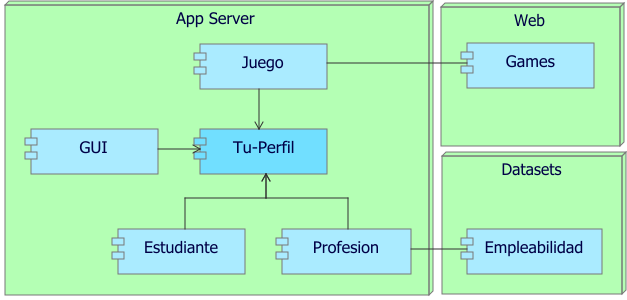
\includegraphics[width=.8\linewidth]{imgs/puntos_vista/tecnologia/uso.pdf}
	\caption{Caso de Uso de la Tecnología}
\end{figure}

Para nuestro caso, en el servidor de aplicaciones vamos a desplegar los componentes descritos en la capa de aplicación, a saber, el componente orquestador Tu-Perfil, los componentes pertenecientes al core de la aplicación, como lo son el componente Profesión, Juego, y Estudiante, además del componente del front, GUI. Por otra parte, se especifican dos componentes externos, el primero de ellos denominado Games, el cual, nos permite integrar juegos online que proporcionan datos sobre las partidas de los juegos y sus correspondientes puntajes en cada una de las modalidades o categorías para ser enviadas y analizadas para el perfilamiento del estudiante. Luego, se especifica el componente Empleabilidad, que nos brinda una estadística sobre las profesiones con mayor demanda en periodos de tiempo ajustables mediante el uso de diferentes datasets. 